%%%%%%%%%%%%%%%%%%%%%%%%%%%%%%%%%%%%%%%%%%%%%%%%%%%%%%%%%%%%%%%%
%%                                                            %%
%% aGreekPrimer, Italian translation 2016.12 - 2017           %%
%%                                                            %%
%% From:  Clarence W. Gleason, A Greek Primer                 %%
%%        (1903, New York, American Book Company)             %%
%%                                                            %%
%%        https://archive.org/details/greekprimer00glea       %%
%%                                                            %%
%% Translated by g.p.ciceri <gp.ciceri@gmail.com>             %%
%% ---------------------------------------------------------- %%
%% This translation is Licensed under                         %%
%% Creative Commons Attribution-ShareAlike 4.0 International  %%
%% https://creativecommons.org/licenses/by-sa/4.0/            %%
%%                                                            %%
%%%%%%%%%%%%%%%%%%%%%%%%%%%%%%%%%%%%%%%%%%%%%%%%%%%%%%%%%%%%%%%%

% ᾶῖῶῆῦ  
% ἀἰὐἐὀὠἠ 
% ὰὲὶὸὺὼὴ 
% ἁἱὑὁὡἡῥ
% άέίόύήώΆΉ
% ἂἒὒἲὂὢἢὒἚἊ
% ἃἳὓὃἣὣἓἋἛ
% ἄἔἴὄὔὤἤἌἬ
% ἅἕἵὅὕὥἥἍἭ
% ἆὦἶἦὖἯἏὯἇὧἷἧὗἯἏὯ 

% ᾳῃῳ
% ᾱῑῡ
% ᾀᾐᾠ
% ᾰῐῠ
% ᾂᾒᾢ
% ϊ ϋ
% ᾄᾔᾤ
% ΰ ΐ
% ᾆᾖᾦ
% ᾲῂῲ
% ᾴῄῴ
% ᾷῇῷ
% ᾳῃῳ
% ᾱῑῡ
% ᾰῐῠ

% āēīōū
% ăĕĭŏŭ

% ᾳῃῳ
% ᾷῇῷ


\documentclass[nols]{tufte-handout}

%\geometry{showframe} % display margins for debugging page layout

\usepackage{fontspec}
\usepackage{ifxetex}
\setmainfont[Path=./fonts/palatino-linotype/, ItalicFont=palai.ttf, BoldFont=palab.ttf]{pala.ttf}
%\setmainfont[Path=./fonts/GFS_Didot/, ItalicFont=GFSDidotItalic.ttf, BoldFont=GFSDidotBold.ttf]{GFSDidot.ttf}

\newfontfamily\GFSDidotBf[Path=./fonts/GFS_Didot/]{GFSDidotBold.ttf}
\newfontfamily\GFSDidot[Path=./fonts/GFS_Didot/]{GFSDidot.ttf}

\newcommand{\didobf}[1]{{\GFSDidotBf #1}}
\newcommand{\dido}[1]{{\GFSDidot #1}}


\usepackage{lipsum}
\usepackage{url}
\usepackage{longtable}
\usepackage{stackengine}

\usepackage{graphicx} % allow embedded images
  \setkeys{Gin}{width=\linewidth,totalheight=\textheight,keepaspectratio}
  \graphicspath{{graphics/}} % set of paths to search for images
\usepackage{amsmath}  % extended mathematics
\usepackage{booktabs} % book-quality tables
\usepackage{units}    % non-stacked fractions and better unit spacing
\usepackage{multicol} % multiple column layout facilities
\usepackage{lipsum}   % filler text
\usepackage{fancyvrb} % extended verbatim environments
  \fvset{fontsize=\normalsize}% default font size for fancy-verbatim environments

% Standardize command font styles and environments
\newcommand{\doccmd}[1]{\texttt{\textbackslash#1}}% command name -- adds backslash automatically
\newcommand{\docopt}[1]{\ensuremath{\langle}\textrm{\textit{#1}}\ensuremath{\rangle}}% optional command argument
\newcommand{\docarg}[1]{\textrm{\textit{#1}}}% (required) command argument
\newcommand{\docenv}[1]{\textsf{#1}}% environment name
\newcommand{\docpkg}[1]{\texttt{#1}}% package name
\newcommand{\doccls}[1]{\texttt{#1}}% document class name
\newcommand{\docclsopt}[1]{\texttt{#1}}% document class option name
\newenvironment{docspec}{\begin{quote}\noindent}{\end{quote}}% command specification environment

% concetti morfosintattici
\usepackage{xspace} 
\newcommand{\noun}{\textsc{sostantivo}\xspace}
\newcommand{\nouns}{\textsc{sostantivi}\xspace}
\newcommand{\adject}{\textsc{aggettivo}\xspace}
\newcommand{\adjects}{\textsc{aggettivi}\xspace}
\newcommand{\gnumber}{\textsc{numero}\xspace}
\newcommand{\gnumbers}{\textsc{numeri}\xspace}
\newcommand{\gender}{\textsc{genere}\xspace}
\newcommand{\genders}{\textsc{generi}\xspace}
\newcommand{\gcase}{\textsc{caso}\xspace}
\newcommand{\gcases}{\textsc{casi}\xspace}
\newcommand{\tense}{\textsc{tempo}\xspace}
\newcommand{\mood}{\textsc{modo}\xspace}
\newcommand{\gverb}{\textsc{verbo}\xspace}
\newcommand{\gverbs}{\textsc{verbi}\xspace}
\newcommand{\adjective}{\textsc{aggettivo}\xspace}
\newcommand{\nom}{\textsc{nom}\xspace}
\newcommand{\gen}{\textsc{gen}\xspace}
\newcommand{\dat}{\textsc{dat}\xspace}
\newcommand{\acc}{\textsc{acc}\xspace}
\newcommand{\voc}{\textsc{voc}\xspace}
\newcommand{\gexit}{\textsc{uscita}\xspace}
\newcommand{\gexits}{\textsc{uscite}\xspace}
\newcommand{\declinazione}{\textsc{declinazione}\xspace}
\newcommand{\masc}{\textsc{maschile}\xspace}
\newcommand{\femm}{\textsc{femminile}\xspace}
\newcommand{\neut}{\textsc{neutro}\xspace}

\newcommand{\indic}{\textsc{indicativo}\xspace}
\newcommand{\imper}{\textsc{imperativo}\xspace}
\newcommand{\gcong}{\textsc{congiuntivo}\xspace}
\newcommand{\ott}{\textsc{ottativo}\xspace}
\newcommand{\partic}{\textsc{participio}\xspace}
\newcommand{\infin}{\textsc{infinito}\xspace}

\newcommand{\pres}{\textsc{presente}\xspace}
\newcommand{\imperf}{\textsc{imperfetto}\xspace}
\newcommand{\aor}{\textsc{aoristo}\xspace}
\newcommand{\fut}{\textsc{futuro}\xspace}
\newcommand{\perf}{\textsc{perfetto}\xspace}
\newcommand{\pperf}{\textsc{piuccheperfetto}\xspace}

\newcommand{\sing}{\textsc{singolare}\xspace}
\newcommand{\plur}{\textsc{plurale}\xspace}
\newcommand{\dual}{\textsc{duale}\xspace}

\newcommand{\si}{\textsc{sing}\xspace}
\newcommand{\pl}{\textsc{plur}\xspace}
\newcommand{\du}{\textsc{dual}\xspace}

\newcommand{\att}{\textsc{attivo}\xspace}
\newcommand{\med}{\textsc{medio}\xspace}
\newcommand{\pass}{\textsc{passivo}\xspace}
\newcommand{\medpass}{\textsc{medio-passivo}\xspace}


% italianitudini
\renewcommand{\figurename}{Figura}
\renewcommand{\tablename}{Tabella}
\renewcommand{\contentsname}{Indice}

% fix per un qualche problema
\ifxetex
  \newcommand{\textls}[2][5]{%
    \begingroup\addfontfeatures{LetterSpace=#1}#2\endgroup
  }
  \renewcommand{\allcapsspacing}[1]{\textls[15]{#1}}
  \renewcommand{\smallcapsspacing}[1]{\textls[10]{#1}}
  \renewcommand{\allcaps}[1]{\textls[15]{\MakeTextUppercase{#1}}}
  \renewcommand{\smallcaps}[1]{\smallcapsspacing{\scshape\MakeTextLowercase{#1}}}
  \renewcommand{\textsc}[1]{\smallcapsspacing{\textsmallcaps{#1}}}
\fi

% too many float...
\extrafloats{100}

\title{A Greek Primer. Introduzione al Greco Antico \newline Lezione XVI - Proclitiche, il pronome \dido{Αὐτός}.}

\author[gpciceri]{a cura di Milagathòs: Milo's help to enjoy humanities}

\date{19 Gennajo 2017} % without \date command, current date is supplied


\begin{document}

\maketitle% this prints the handout title, author, and date

\begin{marginfigure}[-2.0cm]
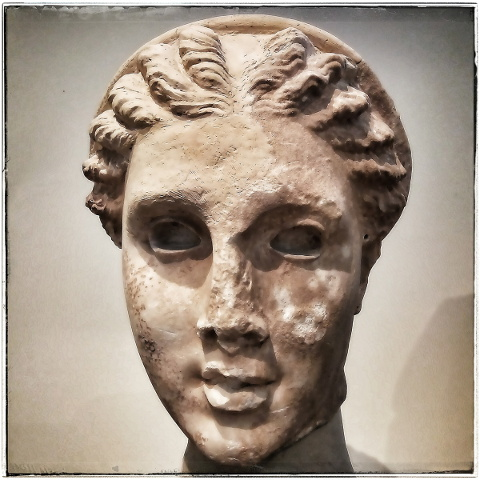
\includegraphics{smallthumb-lesson_XIII.jpeg}
\setfloatalignment{b}
\end{marginfigure}


\begin{abstract}
\noindent
Queste lezioni si articolano in \textsc{elementi grammaticali}, 
espressi sommariamente, seguiti da \textsc{vocabolari} per il lessico di base 
e da \textsc{frasi da tradurre} dal greco e in greco. 
\
L'approccio è quello del testo-laboratorio di morfosintassi: 
si presenta punto per punto - riprendendone la numerazione - 
l'esposizione di Gleason\cite{gleason1903}.\\
\bigskip
\noindent
Lezione XVI: le proclitiche, il pronome \dido{Αὐτός}; vocabolario, esercizi.
\end{abstract}

%\printclassoptions

\newthought{172. Le Proclitiche.} Alcune parole di uso comune non hanno accento e vengono pronunciate assieme alla parola che le segue. Queste parole sono dette \textbf{proclitiche}.\sidenote{da \didobf{προ-κλίνω}, \textit{appoggiarsi in avanti}} 

\newthought{173.} Sono parole proclitiche: le forme dell'articolo \didobf{ὁ, ἡ, οἱ, αἱ}; le congiunzioni \didobf{εἰ}, \textit{se}, \didobf{ὡς}, \textit{come}; l'avverbio di negazione \didobf{οὐ (οὐκ, οὐχ)}, \textit{non}; le preposizioni \didobf{εἰς, ἐν, ἐξ (ἐκ)}.

\newthought{174. Declinazione di \didobf{αὐτός}.} Impara la declinazione di \didobf{αὐτός} (693), confrontandola con quella dell'articolo (692) e del pronome dimostrativo \didobf{οὗτος} (696, XV).

\newthought{(693). Pronome Intensivo \didobf{αὐτός}}

\begin{fullwidth}
\begin{table}[!htbp]
  \centering
  \begin{tabular}{l l l l}
    %\toprule
	\multicolumn{4}{c}{\didobf{αὐτός}, \textsc{stesso, medesimo, egli}} \\
	\multicolumn{4}{c}{\sing} \\
	
	& \masc & \femm & \neut \\
	
	\textsc{n.} & \didobf{αὐτός} & \didobf{αὐτή} & \didobf{αὐτό} \\
	\textsc{g.} & \didobf{αὐτοῦ} & \didobf{αὐτῆς} & \didobf{αὐτοῦ} \\
	\textsc{d.} & \didobf{αὐτῷ} & \didobf{αὐτῇ} & \didobf{αὐτῷ} \\
	\textsc{a.} & \didobf{αὐτόν} & \didobf{αὐτήν} & \didobf{αὐτό} \\
	
	\multicolumn{4}{c}{\plur} \\
	
	& \masc & \femm & \neut \\
	
	\textsc{n.} & \didobf{αὐτοί} & \didobf{αὐταί} & \didobf{αὐτά} \\
	\textsc{g.} & \didobf{αὐτῶν} & \didobf{αὐτῶν} & \didobf{αὐτῶν} \\
	\textsc{d.} & \didobf{αὐτοῖς} & \didobf{αὐταῖς} & \didobf{αὐτοῖς} \\
	\textsc{a.} & \didobf{αὐτούς} & \didobf{αὐτάς} & \didobf{αὐτά} \\
	
	%\bottomrule
  \end{tabular}
  \label{tab:normaltab}
  %\zsavepos{pos:normaltab}
\end{table}
\end{fullwidth}

\newpage

\newthought{(692). Articolo Determinativo \didobf{ὁ, ἡ, τό}}

\begin{fullwidth}
\begin{table}[!htbp]
  \centering
  \begin{tabular}{l l l l}
    %\toprule
	\multicolumn{4}{c}{\didobf{ὁ, ἡ, τό}, \textsc{il, la}} \\
	\multicolumn{4}{c}{\sing} \\
	
	& \masc & \femm & \neut \\
	
	\textsc{n.} & \didobf{ὁ} & \didobf{ἡ} & \didobf{τό} \\
	\textsc{g.} & \didobf{τοῦ} & \didobf{τῆς} & \didobf{τοῦ} \\
	\textsc{d.} & \didobf{τῷ} & \didobf{τῇ} & \didobf{τῷ} \\
	\textsc{a.} & \didobf{τόν} & \didobf{τήν} & \didobf{τό} \\
	
	\multicolumn{4}{c}{\plur} \\
	
	& \masc & \femm & \neut \\
	
	\textsc{n.} & \didobf{οἱ} & \didobf{αἱ} & \didobf{τά} \\
	\textsc{g.} & \didobf{τῶν} & \didobf{τῶν} & \didobf{τῶν} \\
	\textsc{d.} & \didobf{τοῖς} & \didobf{ταῖς} & \didobf{τοῖς} \\
	\textsc{a.} & \didobf{τούς} & \didobf{τάς} & \didobf{τά} \\
	
	%\bottomrule
  \end{tabular}
  \label{tab:normaltab}
  %\zsavepos{pos:normaltab}
\end{table}
\end{fullwidth}

\newthought{175. Frasi Modello} da imparare a memoria.
\begin{itemize}
\item[\textsc{a.}] \didobf{αὐτὸς γὰρ ὁ πατὴρ φιλεῖ ὑμᾶς}, \textit{perché lo stesso padre ti ama.} 
\item[\textsc{b.}] \didobf{τῇ δὲ αὐτῇ νυκτὶ ἧκεν}, \textit{e venne la notte stessa.} 
\item[\textsc{c.}] \didobf{ηὗρον αὐτὸν ἐν τῷ ἱερῷ}, \textit{trovarono lui nel tempio.} 
\end{itemize}

\newthought{Osservazioni}
\begin{itemize}
\item[\textsc{1.}] In \textsc{a.} l'esempio del significato fondamentale di \didobf{αὐτός}, come \textit{ipse} in latino; tuttavia nell'esempio \textsc{b.} \didobf{αὐτός}, quando è preceduto dall'articolo, ha il significato di \textit{idem, medesimo}. 

Osserva come riferimento la posizione di \didobf{αὐτός} relativa all'articolo. \didobf{ὁ νόμος αὐτός}, \textit{la legge stessa (ipse)}. Mentre \didobf{ὁ αὐτὸς νόμος}, \textit{la stessa (medesima, idem) legge}.  
\item[\textsc{2.}] In \textsc{c.} \didobf{αὐτός} è usato come pronome personale. In questo modo \didobf{αὐτός}, mette assieme i significati di \textit{is, ipse} e \textit{idem} 
\end{itemize}

\newthought{176. Vocabolario}

\begin{multicols}{2}
    \noindent \hangindent=1em \didobf{ἔρις, ἔριδος, ἡ} \textit{lotta}.  \\
    \noindent \hangindent=1em \didobf{ξύλον, τό} \textit{legno}.  \\
    \noindent \hangindent=1em \didobf{ὅρκος, ὁ} \textit{giuramento}.  \\
    \noindent \hangindent=1em \didobf{στράτευμα, -ματος, τό} \textit{esercito, armata}.     \\
    \noindent \hangindent=1em \didobf{φόβος, ὁ} \textit{paura}.  \\
		
    \noindent \hangindent=1em \didobf{ἑπτά} agg.indecl. \textit{sette}.  \\
    \noindent \hangindent=1em \didobf{ὀκτώ} agg.indecl. \textit{otto}.  \\
	
    \noindent \hangindent=1em \didobf{αὐτός, αὐτή, αὐτό} agg. e pron. \textit{stesso, medesimo} pron.pers. \textit{egli, quello}.  \\
	
	\noindent \hangindent=1em \didobf{κάω, καύσω, ἔκαυσα, κέκαθκα, +}, \textit{bruciare}.  \\
	
    \noindent \hangindent=1em \didobf{παρ-ἐχω, παρ-ἐξω} e \didobf{παρα-σχήσω, παρ-ἐσχον, παρ-έσχηκα, +}, \textit{fornire, causare, rendere}.  \\
	
	\noindent \hangindent=1em \didobf{περί} prep. con \gen \textit{a proposito, a riguardo}; con \acc \textit{circa, attorno}.  \\
	
	\noindent \hangindent=1em \didobf{ὡς} cong. \textit{come, quando}.  \\
	
\end{multicols}


\newthought{177. Traduci:}
\textsc{1.}~\dido{ὁ δὲ στράτηγὸς αὐτὸς, ἐπεὶ ἔλυσε τὸν ὅρκον, οὐ δίκαιος ἦν.} \quad
\textsc{2.}~\dido{καὶ ἑπτὰ ἡμέρας ἔρις ἦν τοῖς νεανίαις περὶ τούτου.} \quad
\textsc{3.}~\dido{τὰ δὲ στρατεύματα τῶν Θρᾳκῶν παρ-εῖχε\sidenote{in un verbo composto, l'accento non può mai precedere l'aumento. Sia l'aumento che il raddoppiamento vengono dopo la proposizione.} φόβον τοῖς πολεμίοις.} \quad
\textsc{4.}~\dido{καὶ εὐθὺς οἱ φύλακες ἐδίωξαν αὐτοὺς ἐκ τῆς ἄκρας.} \quad
\textsc{5.}~\dido{ἔφυγον δὲ οἱ νεανίαι αὐτοὶ καὶ οἱ κήρυκες σύν αὐτοῖς.} \quad
\textsc{6.}~\dido{ἐντεῦθεν ταχέως ἧκον πλοίοις\sidenote{\dat di mezzo.} εἰς νῆσον μικράν.} \quad
\textsc{7.}~\dido{ὀκτὼ παρασάγγας ἐξ-ήλασε\sidenote{da \didobf{ἐξ-ελαύνω}.} καὶ ἔκαυσε τὰς κώμας.} \quad
\textsc{8.}~\dido{Ξύλα δὲ ἦγον καὶ ἔβαλλον εἰς τὰ πλοῖα.} \quad
\textsc{9.}~\dido{ὡς δὲ ὥρα ἦν δείνου, ἔλαβον ὄσπρια καὶ κρόμμυα ἐκ τῆς ἁμαξης.} \quad
\textsc{10.}~\dido{ἐνταῦθα δὲ ηὗρε διδασκαλεῖον καὶ διδασκάλους· μαθηταὶ δὲ οὐκ ἦσαν.}

\newthought{178. Scrivi in Greco:}
\textsc{1.}~Chi ha rubato gli uccelli? \quad
\textsc{2.}~Li ha gettati nel fiume. \quad
\textsc{3.}~Per cinque giorni il compito fu facile. \quad

\newthought{179. Un epitaffio spartano.}
\\
\centerline{\dido{Ὠ ξεῖν´ ἀγγέλλειν Λακεδαιμονίοις ὅτι τῇδε}} 
\centerline{\dido{κείμεθα, τοῖς κείνων ῥήμασι πειθόμενοι.}}
\centerline{\textit{Dic, hospes, Spartae nos te hic vidisse iacentes}} 
\centerline{\textit{Dum sanctis patriae legibus obsequimur.}}

\begin{figure}[!b]
  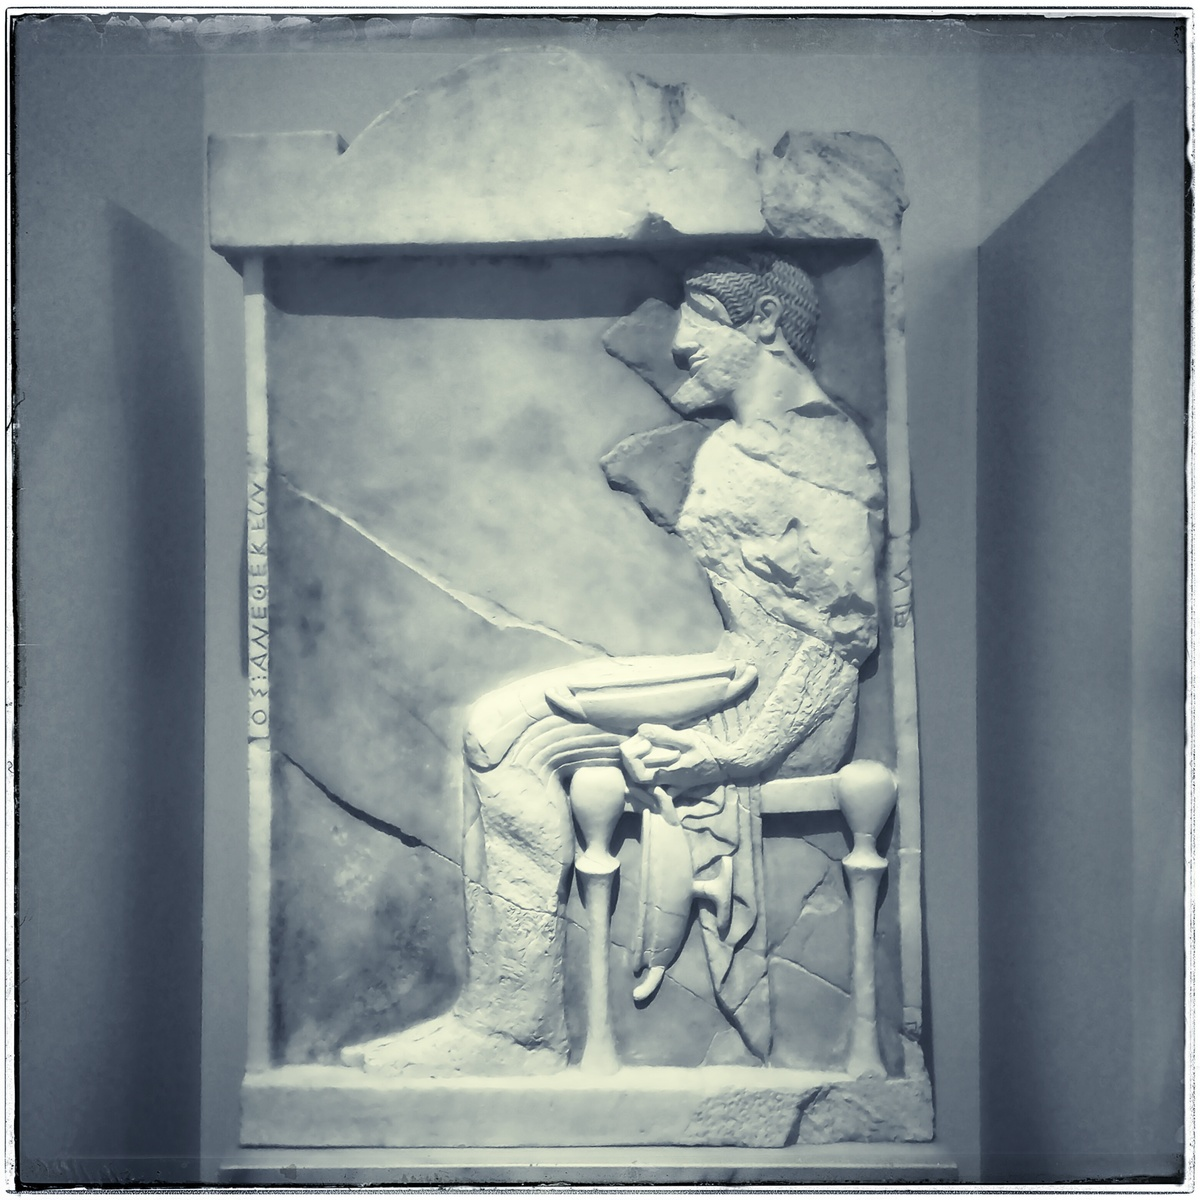
\includegraphics[width=0.8\linewidth]{thumb-lesson_XVI.jpeg}
  %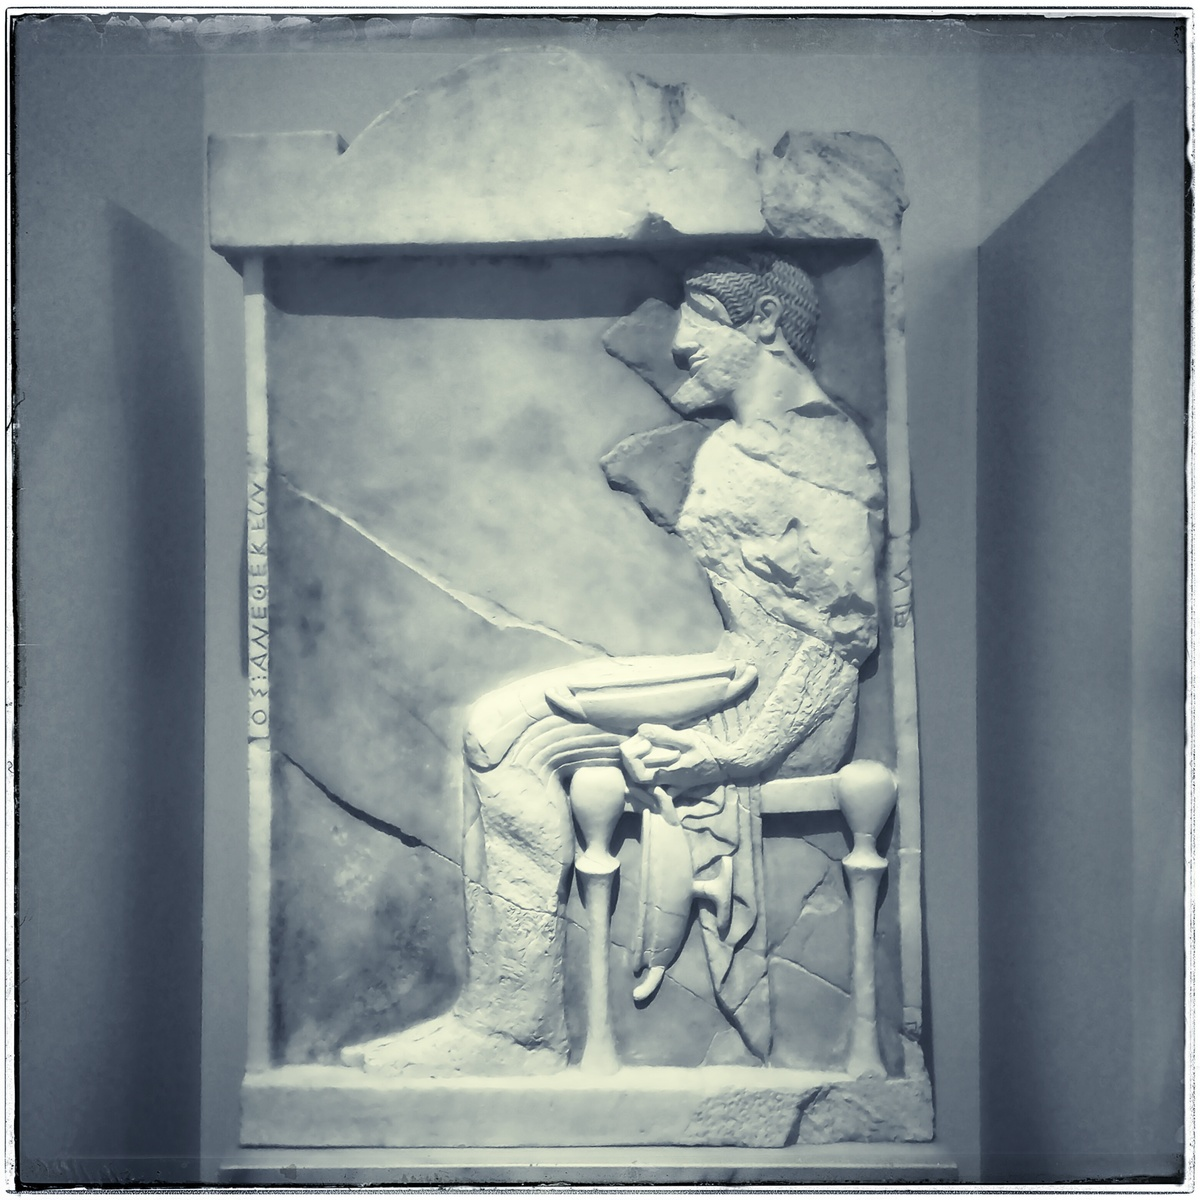
\includegraphics{thumb-lesson_XVI.jpeg}
  \caption{Museo Nazionale di Archeologia di Atene}
  \label{fig:textfig}
  %\zsavepos{pos:textfig}
  %\setfloatalignment{b}
\end{figure}

 

\nobibliography{greekBiblio}
\bibliographystyle{alpha}


\end{document}
